%!TEX TS-program = pdflatex
%!TEX root = tesi.tex
%!TEX encoding = UTF-8 Unicode

\chapter{Introduzione}

\section{Il Problema Affrontato}
In questa tesi si affronta il problema di rilevare la presenza di colla sul fondo di carcasse per motori elettrici, per mezzo di fotografie digitali.
I pezzi da analizzare hanno una forma cilindrica cava con una delle due estremità sigillata.
All'intero della cavità verrà alloggiato un motore elettrico per tergicristalli.
Per poter fissare il motorino è richiesto che un anello di colla sia versato sulla parete verticale interna del pezzo.
Poiché la colla è liquida succede che goccioli fino a raggiungere il fondo del pezzo, questo comporta il malfunzionamento del motore.
Da ciò la necessita di rilevare in modo automatizzato quali pezzi presentano colla sul fondo, così da poterli scartare.

In campo industriale è sempre più frequente che si decida di integrare processi già esistenti con fotocamere per l'acquisizione di immagini.
\todo{magari aggiungere ref}
Le fotocamere, che hanno dimensioni sempre più ridotte ma permettono comunque di scattare fotografie ad ottima risoluzione, possono essere inserite facilmente nella maggior parte dei processi industriali, permettendo di monitorare la produzione senza comprometterla.
Inoltre le immagini raccolte possono andare a formare un \textit{dataset} che, utilizzato per addestrare algoritmi di \textit{machine learning}, permette non solo di monitorare il processo di produzione ma anche di controllarlo.
In questo caso specifico si vuole che il sistema riconosca il maggior numero di carcasse che presentano colla sul fondo, queste verranno poi rimosse automaticamente dal processo di produzione.

Il lavoro svolto in questa tesi nasce per cercare una risposta ad un problema reale.
La soluzione che si propone è stata sviluppata durante un tirocinio, della durata di sei mesi, svolto presso beanTech \footnote{Collegamento al sito ufficiale URL: \url{https://www.beantech.it/}}.
Il principale strumento è stato il linguaggio di programmazione \textit{python}, arricchito da librerie come:
\textit{opencv}\footnote{TODO mettere tutti i bei link?} e \textit{pillow} per la manipolazione e trasformazione delle immagini; 
\textit{numpy} e \textit{scikit-learn} per la gestione di dati numerici;
\textit{pytorch} per tutto ciò che riguarda le reti neurali e convolutive;
\textit{matplotlib} e \textit{pands} per la visualizzazione dei dati.
Per l'allenamento dei modelli si è potuto sfruttare una NVIDIA$^{\text{\textregistered}}$ DGX Station\footnote{https://www.nvidia.com/en-us/data-center/dgx-station/} con quattro NVIDIA$^{\text{\textregistered}}$ TESLA$^{\text{\textregistered}}$ V100 da 32 GB/GPU l'una.
Durante il tirocinio si è sviluppata anche una buona conoscenza dello strumento Docker, che permette di creare spazi virtuali in cui sviluppare, testare e distribuire le proprie soluzioni.

\section{Primi Tentativi}
%Le prime soluzioni proposte si sono rivelate non soddisfacenti, ma poiché fanno parte del percorso che ha portato allo sviluppo della soluzione descritta in questo documento, si è deciso di dedicare un breve commento a quelle più significative.
Le prime soluzioni proposte si sono rivelate non soddisfacenti, ma poiché fanno parte del percorso che ha portato allo sviluppo della soluzione descritta in questo documento, si è deciso di dedicare un breve commento almeno alla prima di queste.

\paragraph{ResNet e One Class SVM} \todo{fix me}
%http://rvlasveld.github.io/blog/2013/07/12/introduction-to-one-class-support-vector-machines/
Come si vedrà meglio poi, il \textit{dataset} è fortemente sbilanciato.
Significa che disponiamo di pochissimi esemplari con colla sul fondo.
La maggior parte dei modelli di \textit{machine learning} per la classificazione viene allenato con almeno due classi.
In questo modo il modello, tramite il confronto, può trovare le caratteristiche che distinguono gli elementi di una classe dall'altra e quindi imparare a riconoscerli.
Quando si dispone di una sola classe ciò non è possibile, bisogna quindi applicare metodi alternativi come la \textit{One Class Support Vector Machine}(OCSVM).
Variazione dell'algoritmo di classificazione \textit{Support Vector Machine}, è stato pensato per poter essere allenato avendo dati di un'unica classe.
Il modo più intuitivo per descrivere il funzionamento di una OCSVM è immaginare che il suo scopo sia creare la più piccola sfera contenente tutti i punti del \textit{dataset}.
Così facendo tutti gli elementi con caratteristiche differenti da quelle degli elementi del \textit{dataset} saranno posizionati a grande distanza dal centro della sfera, probabilmente cadranno all'esterno della sfera.
La classificazione viene effettuata verificando se l'elemento cade entro i confini della sfera, in caso affermativo l'elemento appartiene alla classe utilizzata durante l'allenamento.

\todo[inline]{dire che non si vuole che la OCSVM dia peso ai singoli pixel}
Poiché l'informazione a nostra disposizione è contenuta in immagini si è deciso di usare una rete ResNet18~\cite{resnet} a cui è stato rimosso l'ultimo strato, in questo modo ritornerà vettori di 512 elementi.
Solitamente una rete convolutiva sintetizza i dati contenuti in un'immagine e ritorna il valore della classe più probabile, ma rimuovendo l'ultimo strato si vanno a rimuovere quei neuroni che trasformano un vettore di 512 elementi nel valore della classe più probabile. % TODO non propriamente corretto
Così facendo è possibile, per ogni immagine, ottenere un vettore di dimensioni ridotte.
L'insieme di questi vettori andrà a costituire il \textit{dataset} con cui allenare la OCSVM.

La soluzione appena descritta si è rivelata inadatta ai nostri scopi, fornendo un'accuratezza poco superiore al 60\%, molto inferiore agli obbiettivi che si vogliono raggiungere.

%%\paragraph{Histogram of Oriented Gradients e OCSVM}
%%Si è provato ad ottenere 
%%Un'alternativa alla soluzione precedente 
%
%% tecniche classiche come quella roba della texture
%
%% tecniche classiche come HOG
%
%\paragraph{Manipolazione del Dataset}
%Poiché, dopo svariati tentativi, si è verificato che utilizzare la \textit{One Class SVM} non 
%% immagini a patch
%
%% logpolar immagini

\section{Il Metodo Utilizzato}
La soluzione, che verrà descritta con maggiore dettaglio nelle prossime pagine, sfrutta un particolare tipo di rete neurale che prende il nome di \textit{autoencoder}.
Il funzionamento di un \textit{autoencoder} può essere suddiviso in due momenti:
nel primo i dati in ingresso vengono mappati in uno spazio con dimensionalità inferiore a quella di partenza, si può dire che il dato venga compresso;
nel secondo il dato in forma compressa viene riportato nel suo spazio originale, venendo quindi decompresso.
Un buon \textit{autoencoder} è in grado di fornire in \textit{output} un dato estremamente simile a quello che è stato ricevuto in ingresso, non bisogna pensare però che il suo scopo sia simulare la funzione identità; infatti un compito del genere non sarebbe di alcuna utilità.
L'origine degli autoencoder non è ben definita però ad oggi sono utilizzati per vari scopi.

\paragraph{Dimensionality Reduction}
Sappiamo che gli \textit{autoencoder} possono essere sfruttati per trovare, fissata una dimensionalità, spazi latenti efficaci.
Questa capacità ricorda tecniche di \textit{dimensionality reduction} come la \textit{Principal Component Analysis}(PCA).
Non a caso infatti molti studi, come ad esempio quello intitolato \textit{PCA vs Autoencoders for Dimensionality Reduction}~\cite{pca_vs_ae_1} mettono in luce come gli \textit{autoencoder} siano in grado di equiparare, se non superare, gli approcci classici.
Il principale vantaggio degli \textit{autoencoder} è la possibilità di creare una funzione di compressione specifica per il problema che si vuole risolvere.
Mentre gli approcci come la PCA operano, definita una dimensione da raggiungere, seguendo uno stesso algoritmo per ogni applicazione.

\paragraph{Denoising}
Il \textit{denoising} è una tecnica con cui si rimuove, a partire da un dato non puro, tutta l'informazione considerata rumore.
In figura~\ref{fig:denoise_example} si può vedere come dopo aver introdotto del rumore alle immagini più a sinistra, ottenendo quelle nella seconda colonna, un autoencoder sia in grado di ripristinarle.
L'ultima colonna mostra le immagini generate dalla rete.
\begin{figure}[ht]
  \begin{center}
    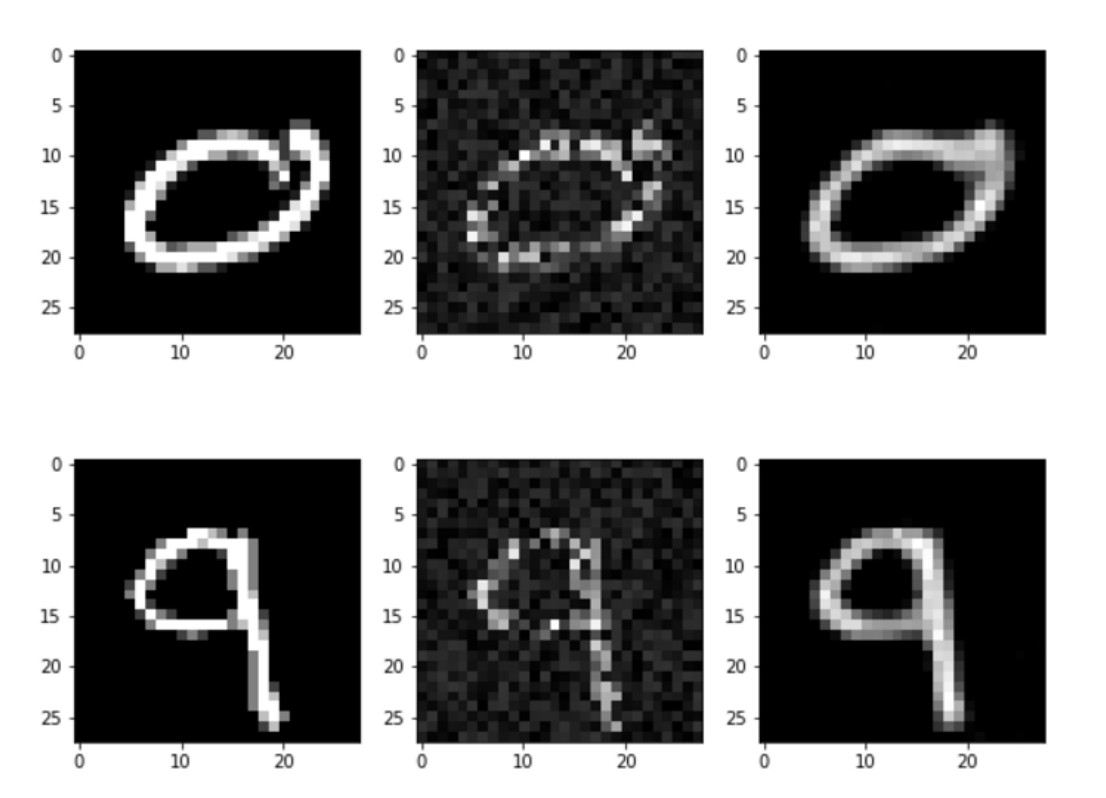
\includegraphics{denoise}
  \end{center}
  \caption{Esempio di applicazione di un \textit{Denoising Autoencoder} URL:\url{http://users.cecs.anu.edu.au/~Tom.Gedeon/conf/ABCs2018/paper/ABCs2018_paper_20.pdf}}
  \label{fig:denoise_example}
\end{figure}
Questo tipo di applicazione può essere sfruttato per effettuare denoising ad immagini di radiografie in campo medico.

%\paragraph{Image Restoration}

\paragraph{Anomaly Detection}
\textit{Anomaly detection} significa letteralmente rilevamento delle anomalie.
Questa tecnica permette, dopo aver definito quali sono i valori attesi, di riconoscere quando i dati ricevuti si allontanano da quelli che ci si aspettava.
Poiché un \textit{autoencoder} può essere facilmente allenato con la classe di valori canonici, imparerà una funzione di compressione adatta a comprimere i valori più frequenti.
Questo significa che la rete fornirà un \textit{output} molto simile a ciò che ha ricevuto in ingresso, se e solo se l'\textit{input} ha caratteristiche simili agli elementi del \textit{dataset}.
Il dato in ingresso, se molto distante dai valori abituali, sarà compresso in un modo che, probabilmente, non ne mantiene le caratteristiche principali.
Ciò comporta, dopo la decompressione, ad ottenere un \textit{output} distante dal dato originale, permettendo di classificare quest'ultimo come anomalia.
